\chapter{Arhitektura i dizajn sustava}

\textnormal{Arhitektura sustava je bazirana na tri komponente koje komuniciraju jedna s drugom. Odnosno, sustav je podijeljen u tri dolje navedena sloja, a koji se mogu prikazati slikom ispod.}
\begin{itemize}
	\item 	\textit{Web poslužitelj}
	\item 	\textit{Web aplikacija}
	\item 	\textit{Baza podataka}
\end{itemize}

\begin{figure}[H]
	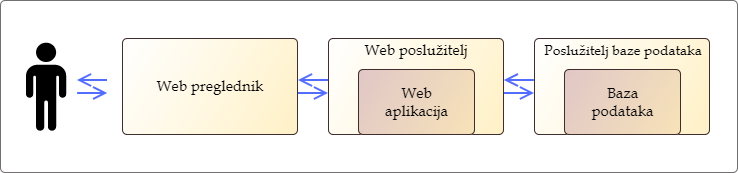
\includegraphics[width=\textwidth]{slike/arhitekturaSustava.png} %veličina slike u odnosu na originalnu datoteku i pozicija slike
	\centering
	\caption{Arhitektura sustava}
	\label{fig:arhitekturasustava}
\end{figure}

\textnormal{\textbf{Web preglednik} omogućava korisniku prikaz web stranice koja pruža određene funkcionalnosti. Omogućava prikaz web stranice (prikaz videa, slika i ostalog multimedijalnog sadržaja) onako kako je definirana u datotekama, dakle omogućuje interpretiranje koda u koristan oblik "običnom" korisniku.
	Putem web preglednika korisnik šalje zahtjev za željenu radnju koja se onda proslijedi idućim koponentama na obradu, te nakon obrade opet se prikazuju u vidljivom obliku kao vid povratne informacije.}

\textnormal{\textbf{Web poslužitelj} je ključna komponenta u obradi korisničkih zahtjeva.
	Dakle, to je \textbf{središnji dio} aplikacije koji omogućava komunikaciju korisnika s aplikacijom.
	U središnjem sloju se odvijaju procesi koji su zaslužni za komunikaciju s bazom podataka ukoliko je to potrebno,
	a to se odvija putem kontrolera, servisa i pristupu bazi podataka.
	U ovom sloju za komunikaciju koristi se Java programski jezik. Odnos komponenti predstavljen je slikom ispod.}

\begin{figure}[H]
	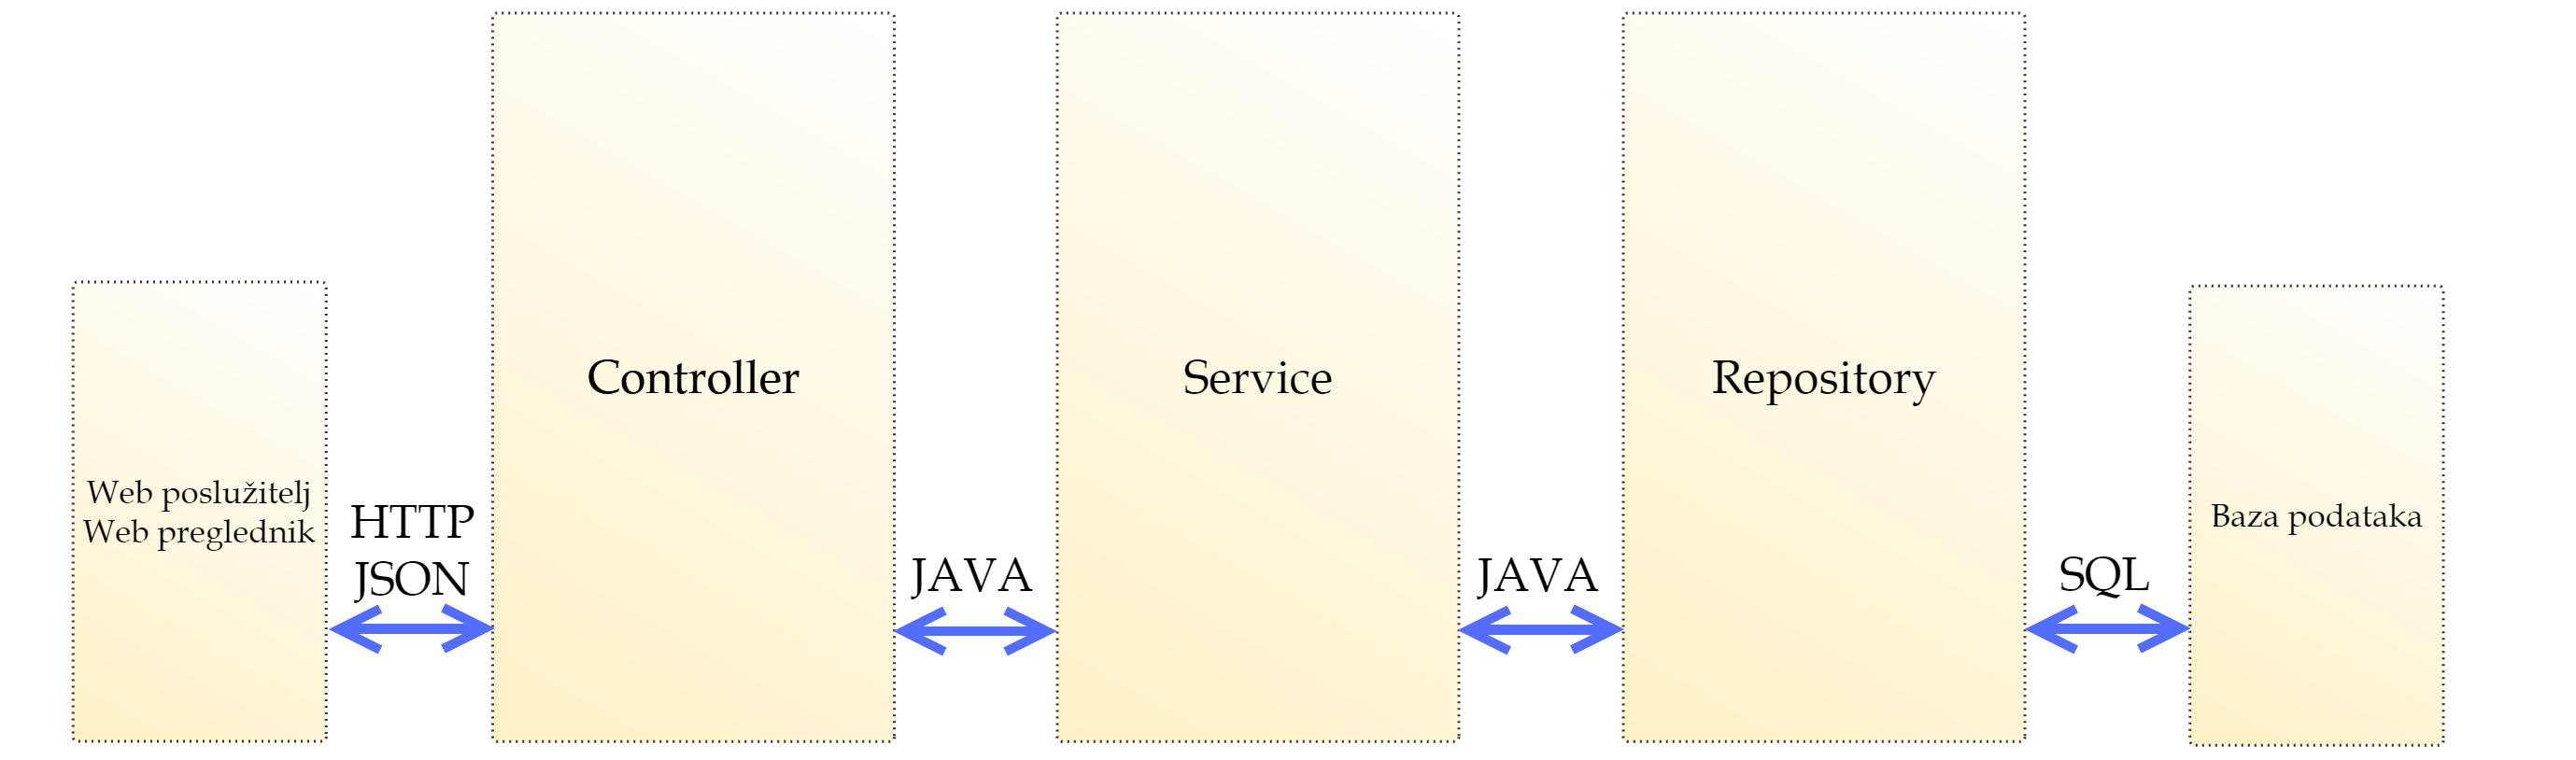
\includegraphics[width=\textwidth]{slike/arhitekturaSustava2.png} %veličina slike u odnosu na originalnu datoteku i pozicija slike
	\centering
	\caption{Arhitektura sustava backend}
	\label{fig:arhitekturasustava2}
\end{figure}

\textnormal{Za izradu ovakve web aplikacije kako bi se pokrile navedene specifične funkcionalnosti koristit će se Spring framework za Javu, te React za prikaz na web pregledniku u radnom okruženju IntelliJIDEA.
	Specifično za Spring framework, koristit će se navedeni tip arhitekture kao što je naveden slikom iznad, jer će se putem metoda JPARepository moći upravljati zahtjevima korisnika koji se vežu za upite u bazi podataka.
	Ukratko, obavljaju se operacije nad \textbf{bazom podataka H2}.}

\textnormal{\textbf{Kontroler} upravlja korisničkim zahtjevima i prosljeđuje ih dalje prema \textbf{Service} gdje se obavlja logika nad upitima i zahtjevima. Service komunicira s \textbf{bazom podataka} preko JPARepository.}

\textnormal{UI će biti povezan sa ostalim dijelovima web aplikacije putem \textbf{REST servisa}, odnosno REST servis komunicira s navedena tri sloja: Controller, Service i Repository. Takva vrsta komunikacije je predstavljena idućom slikom.
	UI je izveden uz pomoć \textbf{React} framework-a koji se koristi komponentama za organizaciju prikaza.}

\begin{figure}[H]
	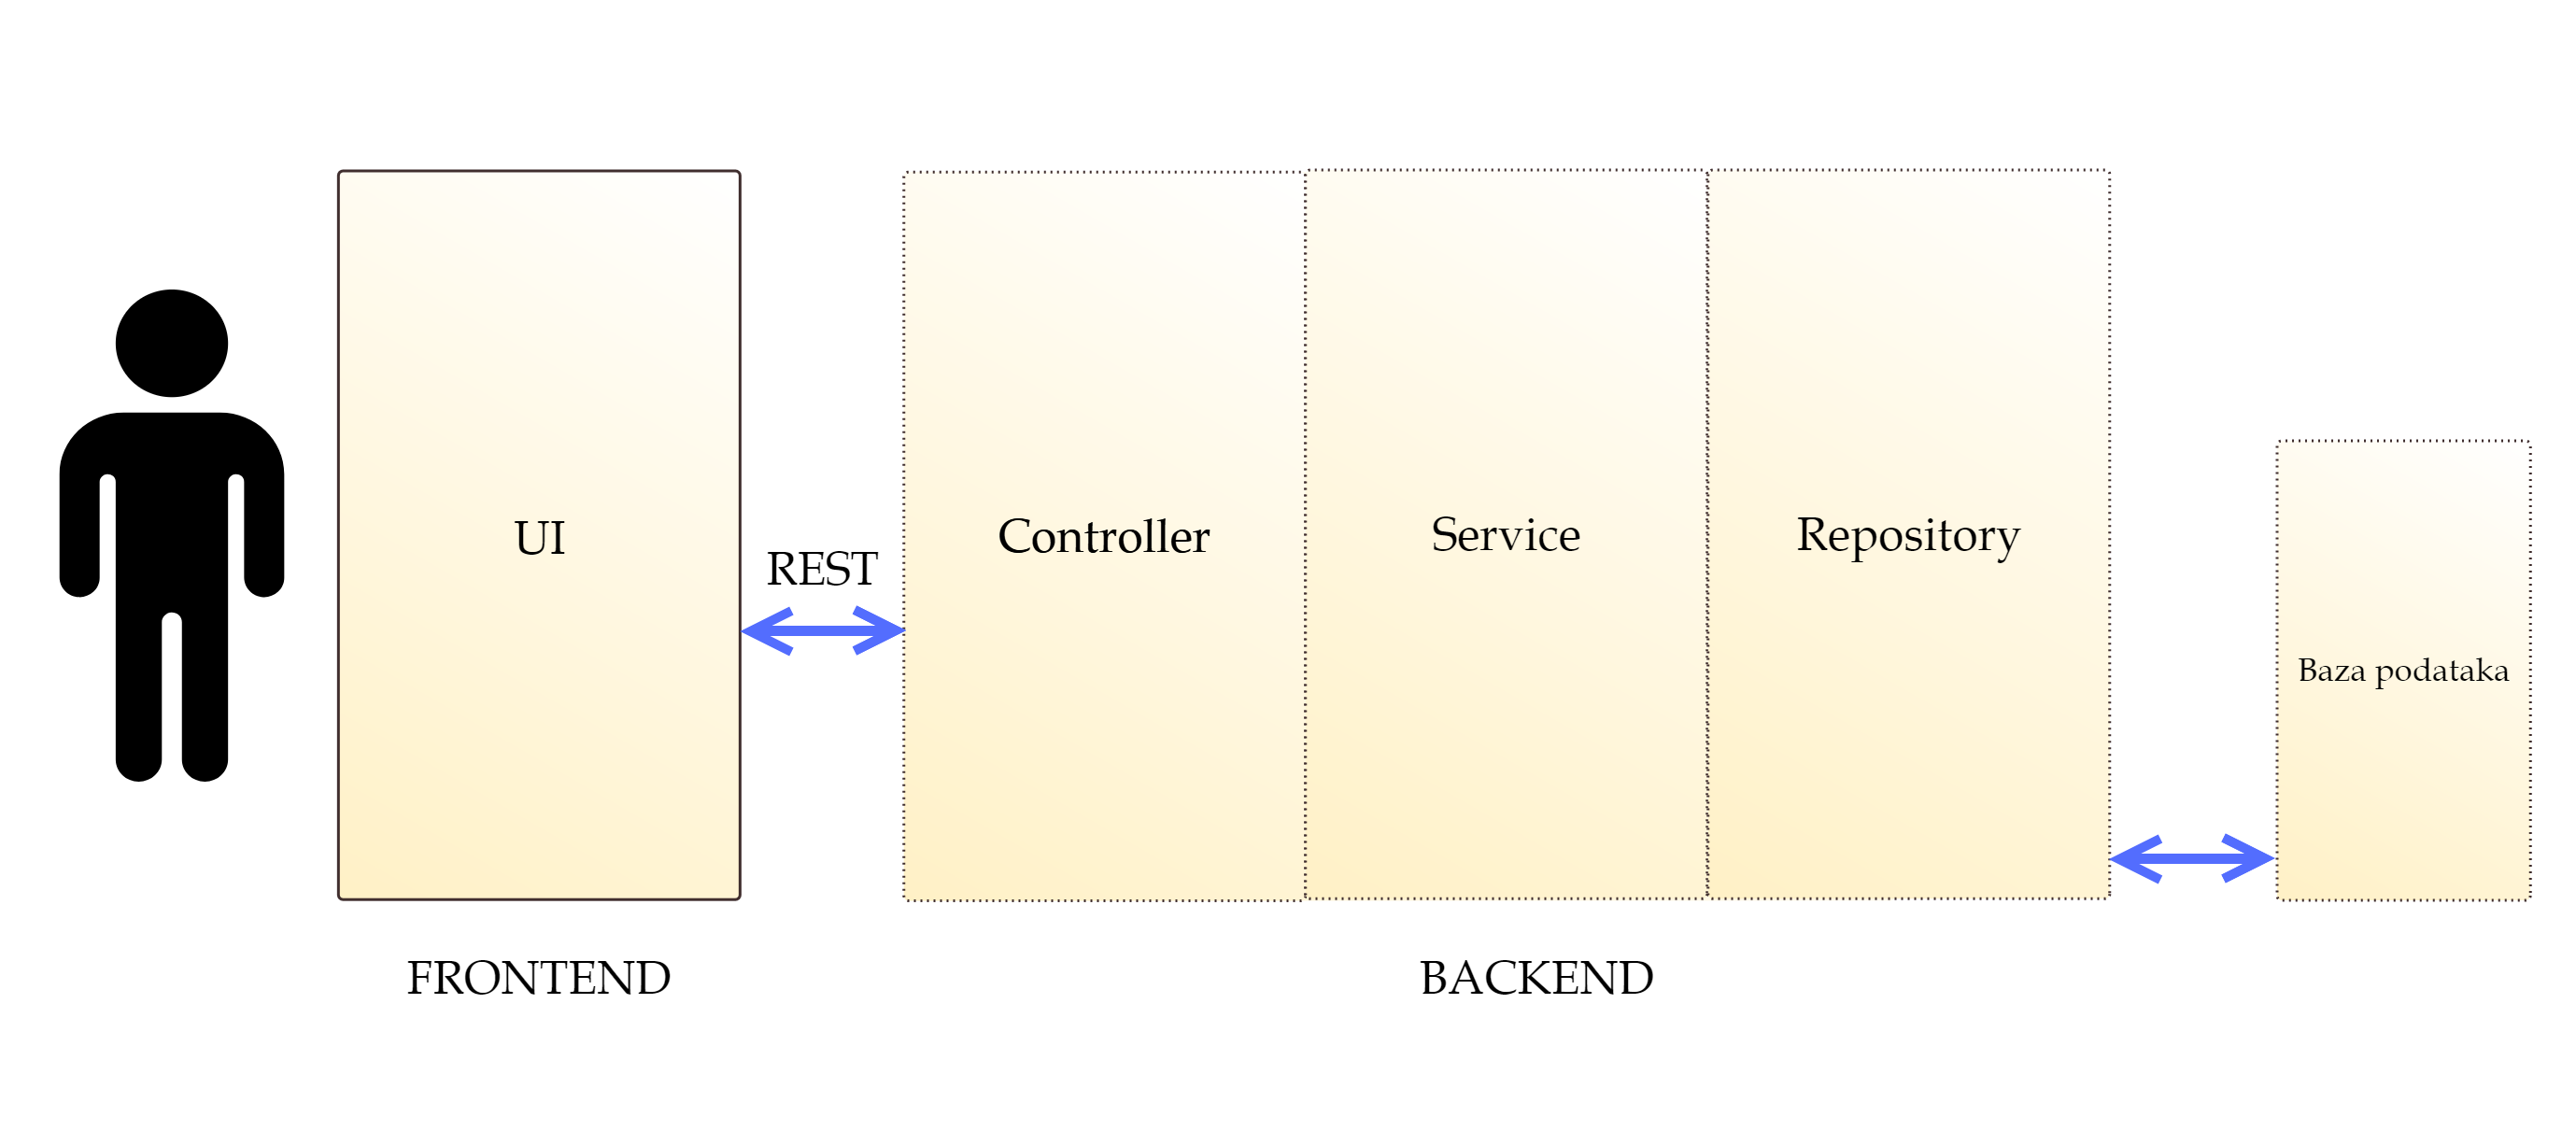
\includegraphics[width=\textwidth]{slike/arhitekturaSustava3.png} %veličina slike u odnosu na originalnu datoteku i pozicija slike
	\centering
	\caption{Arhitektura sustava backend i frontend}
	\label{fig:arhitekturasustava3}
\end{figure}

\eject





\section{Baza podataka}


\textnormal{Kao rješenje za web aplikaciju koju izrađujemo, odlučili smo se na relacijski model baze podataka jer nam ona omogućava precizno oblikovanje i modeliranje elemenata iz stvarnog svijeta. Međusobni odnos tablica se zasniva na relaciji dok se svaka tablica sastoji od naziva entiteta te njegovih pripadajućih atributa koji opisuju dani entitet. Ovakav tip baze podataka u ovom slučaju nam omogućava brzo spremanje, dohvat i izmjenu (uređivanje ili brisanje) podataka koji cirkulišu u web aplikaciji. Baza podataka koja je spremna za izradu ove web aplikacije se sastoji od sljedećih elemenata/tablica:}

\begin{packed_item}

	\item Korisnik
	\item Recept
	\item Video
	\item Objava
	\item Kategorija
	\item ReceptKategorije
	\item ReceptSastojci
	\item Sastojak
	\item Komentar
	\item OmiljeniAutor
	\item OznačenRecept
	\item SpremljenRecept
	\item VrstaKuhinja
	\item Obavijesti

\end{packed_item}

\eject

\subsection{Opis tablica}


\textnormal{\textbf{Korisnik}		Entitet Korisnik služi za evidenciju podataka o korisnicima koji koriste web aplikaciju. Atributi koji ga opisuju su korisnickoIme, lozinkaKorisnik, imeKorisnik, prezimeKorisnik, brojTelefona, emailKorisnik, razinaOvlasti i Dostupan što označava kada je dostupan za komunikaciju s drugim korisnicima unutar web aplikacije. Entitet Korisnik je u \textit{One-To-Many} vezi s entitetom Recept. Entitet Korisnik je i u \textit{Many-To-Many} vezi s entitetom OmiljeniAutor koji bilježi korisnike koje ovaj korisnik prati. Također, ovaj entitet je u \textit{Many-To-Many} vezi s entitetima SpremljenRecept, OznačenRecept, a u \textit{One-To-Many} vezi s entitetima Objava i Komentar.}


\begin{longtblr}[
	label=none,
	entry=none
	]{
	width = \textwidth,
	colspec={|X[8,l]|X[6, l]|X[20, l]|},
	rowhead = 1,
	} %definicija širine tablice, širine stupaca, poravnanje i broja redaka naslova tablice
	\hline \SetCell[c=3]{c}{\textbf{Korisnik}}                                     \\ \hline[3pt]
	\SetCell{LightGreen}IDKorisnik & INT     & jedinstveni identifikator korisnika \\ \hline
	KorisnickoIme                  & VARCHAR & korisničko ime                      \\ \hline
	LozinkaKorisnik                & VARCHAR & spremljena hash lozinka za pristup  \\ \hline
	ImeKorisnik                    & VARCHAR & ime korisnika                       \\ \hline
	PrezimeKorisnik                & VARCHAR & prezime korisnika                   \\ \hline
	BrojTelefona                   & VARCHAR & broj telefona korisnika             \\ \hline
	EmailKorisnik                  & VARCHAR & e-mail adresa korisnika             \\ \hline
	RazinaOvlasti                  & VARCHAR & razina ovlasti u aplikaciji         \\ \hline
	Dostupan                       & TIME    & vrijeme dostupnosti                 \\ \hline
\end{longtblr}

\eject

\textnormal{\textbf{Komentar}		Entitet Komentar služi za evidenciju komentara koji korisnici međusobno dijele u web aplikaciji. Opisuju ga atributi IDKomentar, IDKorisnik, IDObjava, te NaslovKomentar, SadrzajKomentar i DatumKomentar. Ovaj entitet je  u \textit{Many-To-One} vezi s entitetom Korisnik, te u istoj vezi s entitetom Objava.}

\begin{longtblr}[
	label=none,
	entry=none
	]{
	width = \textwidth,
	colspec={|X[8,l]|X[6, l]|X[20, l]|},
	rowhead = 1,
	} %definicija širine tablice, širine stupaca, poravnanje i broja redaka naslova tablice
	\hline \SetCell[c=3]{c}{\textbf{Komentar}}                                     \\ \hline[3pt]
	\SetCell{LightGreen}IDKomentar & INT     & jedinstveni identifikator komentara \\ \hline
	IDKorisnik                     & INT     & jedinstveni identifikator korisnika \\ \hline
	IDObjava                       & INT     & jedinstveni identifikator objave    \\ \hline
	NaslovKomentar                 & VARCHAR & naziv komentara                     \\ \hline
	OpisKomentar                   & VARCHAR & sadržaj komentara                   \\ \hline
	DatumKomentar                  & DATE    & datum komentara                     \\ \hline
\end{longtblr}


\vspace{\baselineskip}
\textnormal{\textbf{OmiljeniAutor}		Entitet OmiljeniAutor služi za evidenciju korisnika koje jedan korisnik zaprati. Opisan je sljedećim atributima: IDKorisnik i IDAutor. U \textit{Many-To-Many} je vezi s entitetom Korisnik unutar web aplikacije.}

\begin{longtblr}[
	label=none,
	entry=none
	]{
	width = \textwidth,
	colspec={|X[6,l]|X[6, l]|X[20, l]|},
	rowhead = 1,
	} %definicija širine tablice, širine stupaca, poravnanje i broja redaka naslova tablice
	\hline \SetCell[c=3]{c}{\textbf{OmiljeniAutor}}                             \\ \hline[3pt]
	\SetCell{LightGreen}IDKorisnik & INT & jedinstveni identifikator pratitelja \\ \hline
	IDAutor                        & INT & ID korisnika koji je zapraćen        \\ \hline
\end{longtblr}

\vspace{\baselineskip}
\textnormal{\textbf{Recept}		Entitet Recept služi za evidenciju podataka o receptima koji cirkulišu i nastaju u web aplikaciji. Opisan je atributima: IDRecept, NazivRecept, IDKategorija, IDSastojak, IDVrstaKuhinja, PripremaRecept, VrijemeKuhanja, IDOznaka, SlikaRecept i IDVideoRecept. Entitet Recept je u \textit{Many-To-One} vezi s entitetom Korisnik, a u \textit{Many-To-Many} vezi s entitetom Sastojak, te u \textit{Many-To-Many} vezi s Kategorija, a \textit{One-To-One} s VrstaKuhinja. Također je u \textit{One-To-One} vezi s entitetom Objava.}

\begin{longtblr}[
	label=none,
	entry=none
	]{
	width = \textwidth,
	colspec={|X[8,l]|X[6, l]|X[20, l]|},
	rowhead = 1,
	} %definicija širine tablice, širine stupaca, poravnanje i broja redaka naslova tablice
	\hline \SetCell[c=3]{c}{\textbf{Recept}}                                      \\ \hline[3pt]
	\SetCell{LightGreen}IDRecept & INT     & jedinstveni identifikator recepta    \\ \hline
	NazivRecept                  & VARCHAR & naziv recepta                        \\ \hline
	IDKategorija                 & INT     & ID kategorije kojoj recept pripada   \\ \hline
	IDSastojak                   & INT     & ID sastojka u receptu                \\ \hline
	IDVrstaKuhinja               & INT     & ID vrste kuhinje recepta             \\ \hline
	PripremaRecept               & VARCHAR & Opis pripreme recepta                \\ \hline
	VrijemeKuhanja               & TIME    & Vrijeme potrebno za pripremu recepta \\ \hline
	IDOznaka                     & INT     & ID oznake recepta                    \\ \hline
	SlikaRecept                  & VARCHAR & Slika recepta                        \\ \hline
	IDVideoRecept                & INT     & ID Video recepta                     \\ \hline
\end{longtblr}

\vspace{\baselineskip}
\textnormal{\textbf{Video}		Entitet Video služi za evidenciju videa koji se objavljuju uz recepte. Opisan je sljedećim atributima: IDVideo, NazivVideo i TrajanjeVideo što omogućuje pretragu recepata po dužini pripremanja. U \textit{One-To-One} je vezi s entitetom Recept unutar web aplikacije.}

\begin{longtblr}[
	label=none,
	entry=none
	]{
	width = \textwidth,
	colspec={|X[6,l]|X[6, l]|X[20, l]|},
	rowhead = 1,
	} %definicija širine tablice, širine stupaca, poravnanje i broja redaka naslova tablice
	\hline \SetCell[c=3]{c}{\textbf{Video}}                                 \\ \hline[3pt]
	\SetCell{LightGreen}IDVideo & INT     & jedinstveni identifikator videa \\ \hline
	NazivVideo                  & VARCHAR & naziv videa                     \\ \hline
	TrajanjeVideo               & TIME    & trajanje videa                  \\ \hline
\end{longtblr}

\vspace{\baselineskip}
\textnormal{\textbf{Objava}		Entitet Objava služi za evidenciju objava recepata koje korisnici objavljuju unutar web aplikacije. Opisan je atributima: IDObjava, IDKorisnik, IDRecept i DatumObjava. U \textit{Many-To-One} vezi je s entitetom Korisnik, te u \textit{Many-To-Many} vezi s entitetom Komentar i u \textit{One-To-One} s entitetom Recept.}

\begin{longtblr}[
	label=none,
	entry=none
	]{
	width = \textwidth,
	colspec={|X[6,l]|X[6, l]|X[20, l]|},
	rowhead = 1,
	} %definicija širine tablice, širine stupaca, poravnanje i broja redaka naslova tablice
	\hline \SetCell[c=3]{c}{\textbf{Objava}}                                  \\ \hline[3pt]
	\SetCell{LightGreen}IDObjava & INT  & jedinstveni identifikator objave    \\ \hline
	IDKorisnik                   & INT  & jedinstveni identifikator korisnika \\ \hline
	IDRecept                     & INT  & jedinstveni identifikator recepta   \\ \hline
	DatumObjava                  & DATE & datum objave                        \\ \hline
\end{longtblr}

\vspace{\baselineskip}
\textnormal{\textbf{OznačenRecept}		Entitet OznačenRecept služi za evidenciju označenih recepata od strane korisnika. Opisan je atributima: IDRecept i IDKorisnik. U \textit{Many-To-Many} vezi je s entitetom Korisnik.}

\begin{longtblr}[
	label=none,
	entry=none
	]{
	width = \textwidth,
	colspec={|X[6,l]|X[6, l]|X[20, l]|},
	rowhead = 1,
	} %definicija širine tablice, širine stupaca, poravnanje i broja redaka naslova tablice
	\hline \SetCell[c=3]{c}{\textbf{OznačenRecept}}                          \\ \hline[3pt]
	\SetCell{LightGreen}IDRecept & INT & jedinstveni identifikator recepta   \\ \hline
	IDKorisnik                   & INT & ID korisnika koji je označio recept \\ \hline
\end{longtblr}

\vspace{\baselineskip}
\textnormal{\textbf{SpremljenRecept}		Entitet SpremljenRecept za evidenciju spremljenih recepata od strane korisnika. Opisan je atributima: IDRecept i IDKorisnik. U \textit{Many-To-Many} vezi je s entitetom Korisnik.}

\begin{longtblr}[
	label=none,
	entry=none
	]{
	width = \textwidth,
	colspec={|X[6,l]|X[6, l]|X[20, l]|},
	rowhead = 1,
	} %definicija širine tablice, širine stupaca, poravnanje i broja redaka naslova tablice
	\hline \SetCell[c=3]{c}{\textbf{SpremljenRecept}}                        \\ \hline[3pt]
	\SetCell{LightGreen}IDRecept & INT & jedinstveni identifikator recepta   \\ \hline
	IDKorisnik                   & INT & ID korisnika koji je spremio recept \\ \hline
\end{longtblr}

\vspace{\baselineskip}
\textnormal{\textbf{Kategorija}		Entitet Kategorija služi za evidenciju kategorija. Opisan je atributima: IDKategorija, NazivKategorija i OpisKategorija.}

\begin{longtblr}[
	label=none,
	entry=none
	]{
	width = \textwidth,
	colspec={|X[8,l]|X[6, l]|X[20, l]|},
	rowhead = 1,
	} %definicija širine tablice, širine stupaca, poravnanje i broja redaka naslova tablice
	\hline \SetCell[c=3]{c}{\textbf{Kategorija}}                                      \\ \hline[3pt]
	\SetCell{LightGreen}IDKategorija & INT     & jedinstveni identifikator kateogrije \\ \hline
	NazivKategorija                  & VARCHAR & naziv kategorije                     \\ \hline
	OpisKategorija                   & VARCHAR & opis kategorije                      \\ \hline
\end{longtblr}

\vspace{\baselineskip}
\textnormal{\textbf{ReceptKategorije}		Entitet ReceptKategorije služi za evidenciju kategorija i recepata pod tim kategorijama. Opisan je atributima: IDKategorija, NazivKategorija i OpisKategorija. U \textit{Many-To-Many} vezi je s entitetom Recept.}

\begin{longtblr}[
	label=none,
	entry=none
	]{
	width = \textwidth,
	colspec={|X[8,l]|X[6, l]|X[20, l]|},
	rowhead = 1,
	} %definicija širine tablice, širine stupaca, poravnanje i broja redaka naslova tablice
	\hline \SetCell[c=3]{c}{\textbf{ReceptKategorije}}                        \\ \hline[3pt]
	\SetCell{LightGreen}IDRecept & INT & jedinstveni identifikator kateogrije \\ \hline
	IDKategorija                 & INT & jedinstveni identifikator recepta    \\ \hline
\end{longtblr}

\vspace{\baselineskip}
\textnormal{\textbf{VrstaKuhinja}		Entitet VrstaKuhinja služi za evidenciju različitih vrsta kuhinja. Opisan je atributima: IDVrstaKuhinja, NazivVrstaKuhinja i OpisKategorija. U \textit{One-To-One} vezi je s entitetom Recept.}

\begin{longtblr}[
	label=none,
	entry=none
	]{
	width = \textwidth,
	colspec={|X[9,l]|X[6, l]|X[20, l]|},
	rowhead = 1,
	} %definicija širine tablice, širine stupaca, poravnanje i broja redaka naslova tablice
	\hline \SetCell[c=3]{c}{\textbf{VrstaKuhinja}}                                         \\ \hline[3pt]
	\SetCell{LightGreen}IDVrstaKuhinje & INT     & jedinstveni identifikator vrste kuhinje \\ \hline
	NazivVrstaKuhinja                  & VARCHAR & naziv vrste kuhinje                     \\ \hline
\end{longtblr}

\vspace{\baselineskip}
\textnormal{\textbf{Sastojak}		Entitet Sastojak služi za evidenciju različitih sastojaka. Opisan je atributima: IDSastojak, NazivSastojak.}

\begin{longtblr}[
	label=none,
	entry=none
	]{
	width = \textwidth,
	colspec={|X[6,l]|X[6, l]|X[20, l]|},
	rowhead = 1,
	} %definicija širine tablice, širine stupaca, poravnanje i broja redaka naslova tablice
	\hline \SetCell[c=3]{c}{\textbf{Sastojak}}                                    \\ \hline[3pt]
	\SetCell{LightGreen}IDSastojak & INT     & jedinstveni identifikator sastojka \\ \hline
	NazivSastojak                  & VARCHAR & naziv sastojka                     \\ \hline
\end{longtblr}

\vspace{\baselineskip}
\textnormal{\textbf{ReceptSastojci}		Entitet ReceptSastojci služi za evidenciju različitih sastojaka unutar recepta. Opisan je atributima: IDRecept, IDSastojak i KolicinaSastojak. U \textit{Many-To-Many} vezi je s entitetom Recept.}

\begin{longtblr}[
	label=none,
	entry=none
	]{
	width = \textwidth,
	colspec={|X[8,l]|X[6, l]|X[20, l]|},
	rowhead = 1,
	} %definicija širine tablice, širine stupaca, poravnanje i broja redaka naslova tablice
	\hline \SetCell[c=3]{c}{\textbf{ReceptSastojci}}                            \\ \hline[3pt]
	\SetCell{LightGreen}IDRecept & INT     & jedinstveni identifikator recepta  \\ \hline
	IDSastojak                   & INT     & jedinstveni identifikator sastojka \\ \hline
	KolicinaSastojak             & VARCHAR & količina sastojka                  \\ \hline
\end{longtblr}

\vspace{\baselineskip}
\textnormal{\textbf{Obavijesti}		Entitet Obavijesti služi za slanje obavijesti korisnicima koji prate određene autore recepata. Opisan je atributima: IDObavijest, IDAutor, NazivObavijest, SadrzajObavijest, DatumObavijest i JeProcitano. U \textit{Many-To-One} vezi je s entitetom Korisnik.}

\begin{longtblr}[
	label=none,
	entry=none
	]{
	width = \textwidth,
	colspec={|X[8,l]|X[6, l]|X[20, l]|},
	rowhead = 1,
	} %definicija širine tablice, širine stupaca, poravnanje i broja redaka naslova tablice
	\hline \SetCell[c=3]{c}{\textbf{Obavijesti}}                                    \\ \hline[3pt]
	\SetCell{LightGreen}IDObavijest & INT     & jed. identifikator obavijesti       \\ \hline
	IDKorisnik                      & INT     & jedinstveni identifikator korisnika \\ \hline
	NazivObavijest                  & VARCHAR & naziv obavijesti                    \\ \hline
	SadrzajObavijest                & VARCHAR & sadržaj obavijesti                  \\ \hline
	DatumObavijest                  & DATE    & datum obavijesti                    \\ \hline
	JeProcitano                     & TINYINT & oznaka pročitane obavijesti         \\ \hline
\end{longtblr}

\subsection{Dijagram baze podataka}
%unos slike
\begin{figure}[H]
	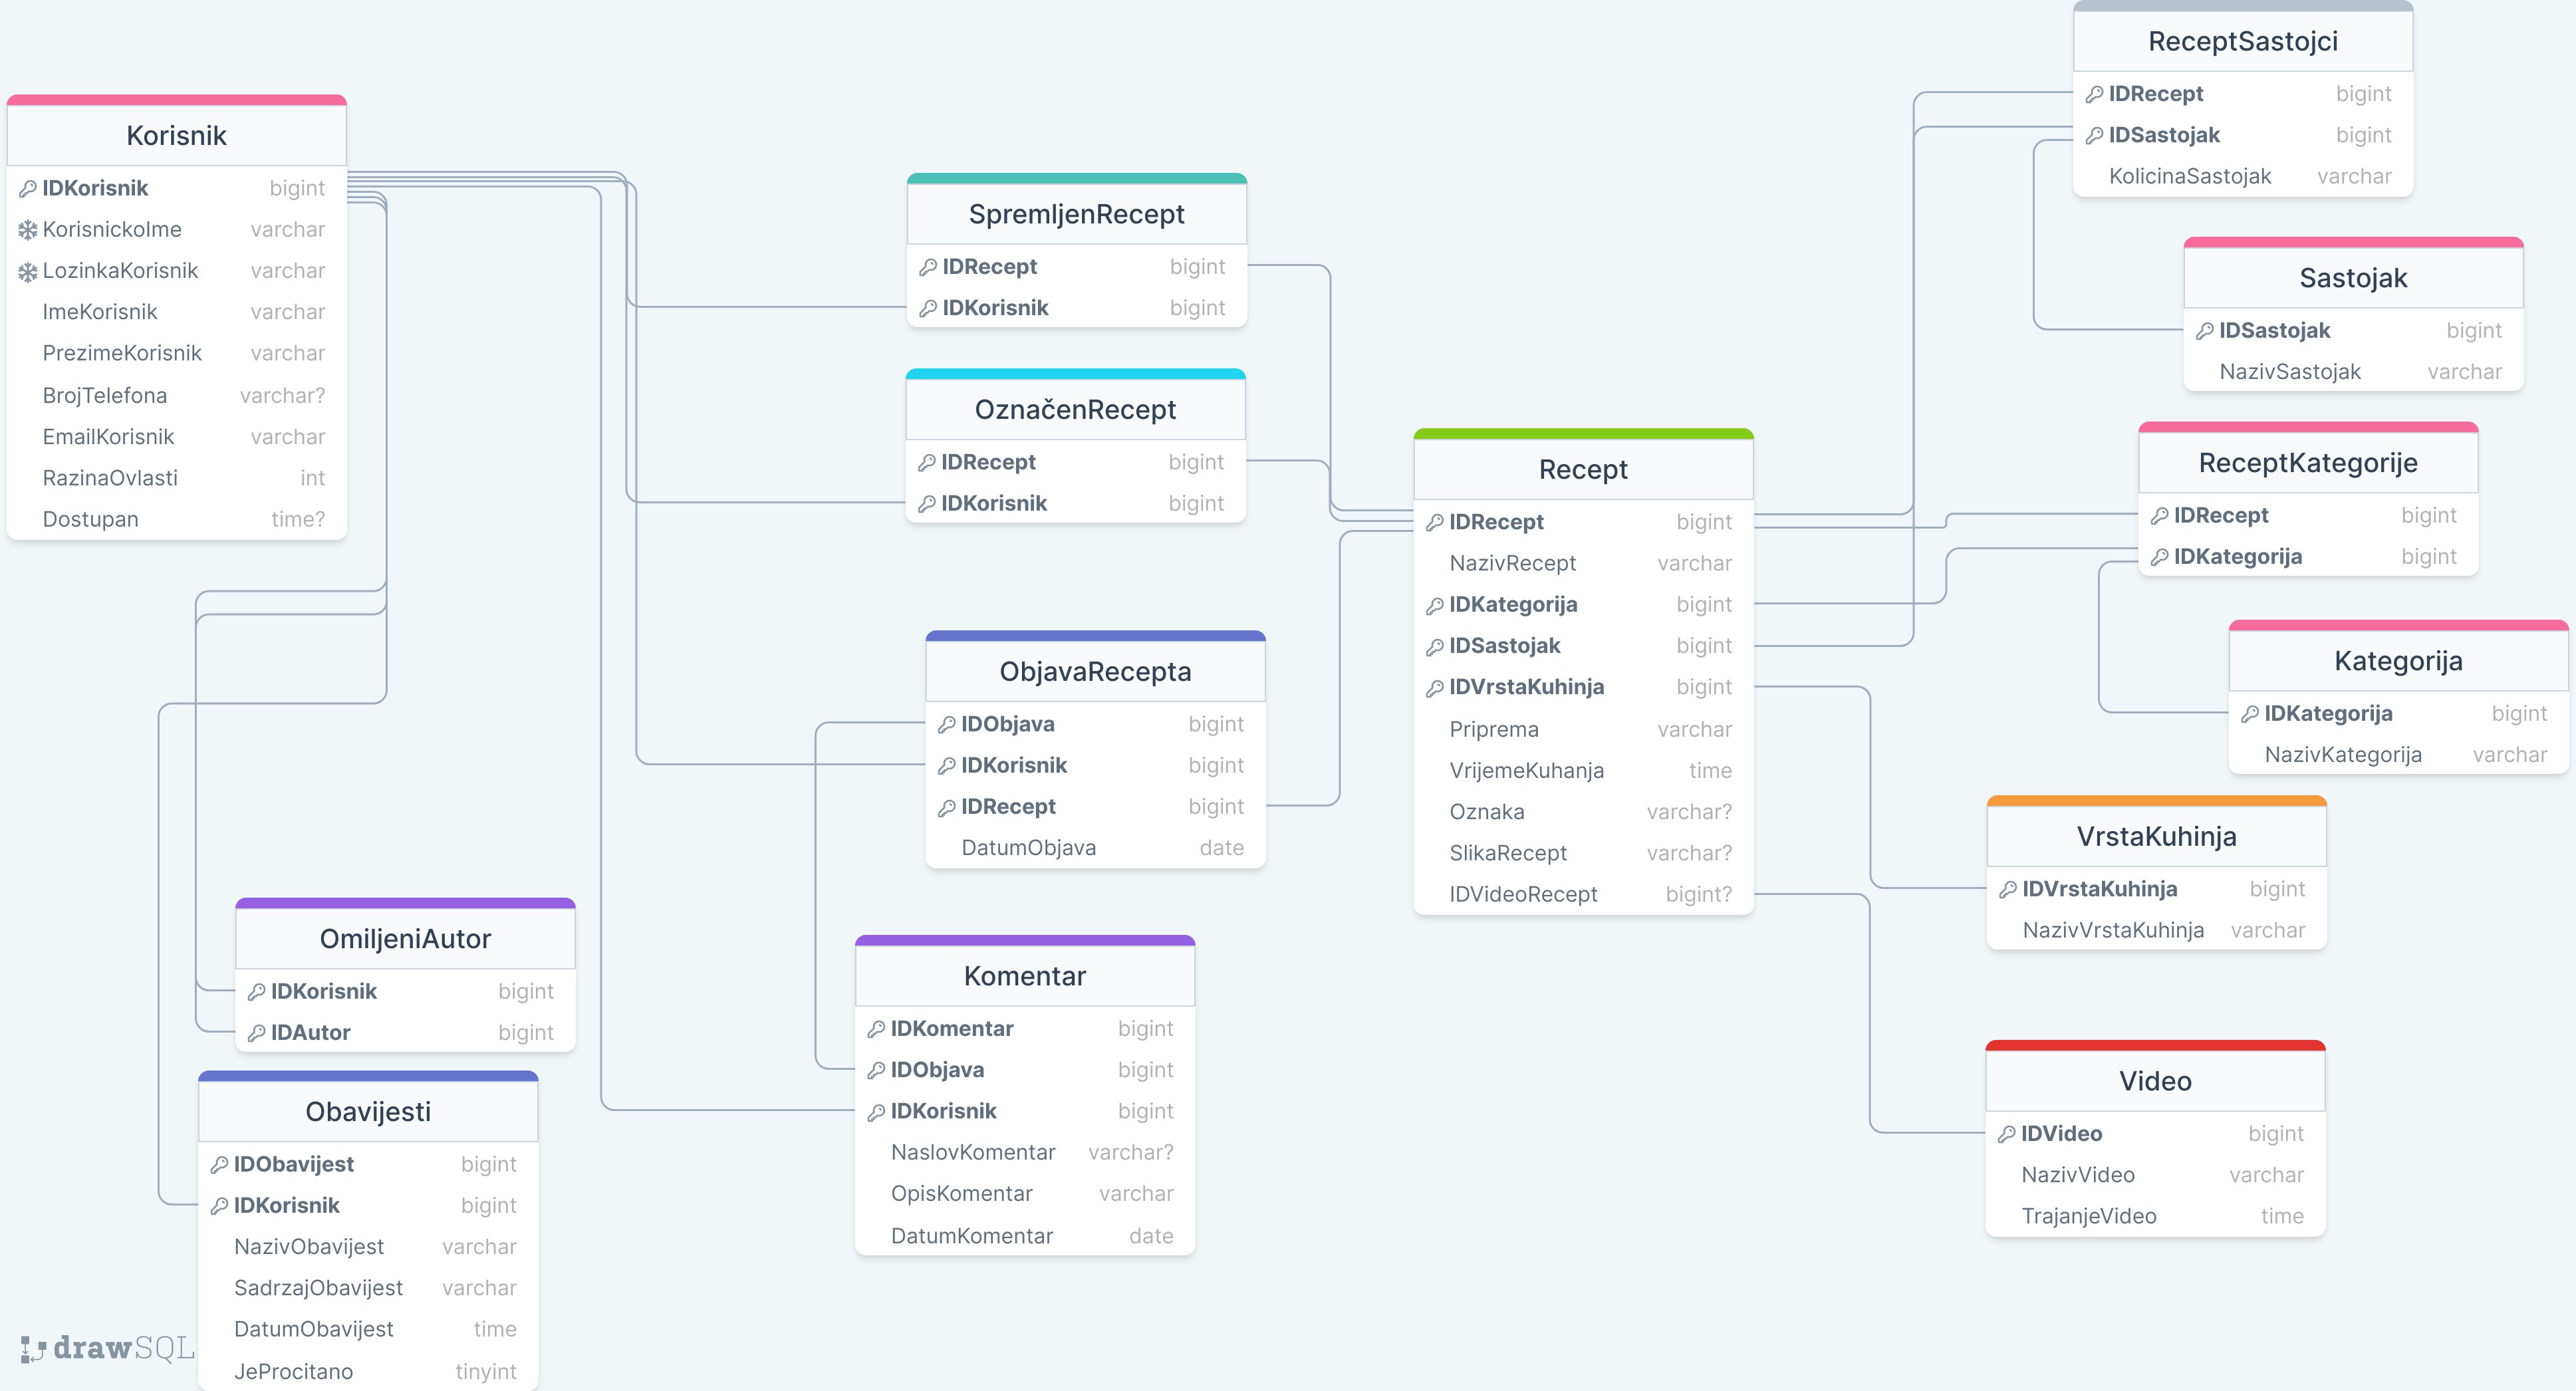
\includegraphics[width=\textwidth]{slike/CookBooked-dbp.png} %veličina slike u odnosu na originalnu datoteku i pozicija slike
	\centering
	\caption{Dijagram relacijske baze podataka za web aplikaciju}
	\label{fig:dijagrambp}
\end{figure}
\eject


\section{Dijagram razreda}

\begin{figure}[H]
	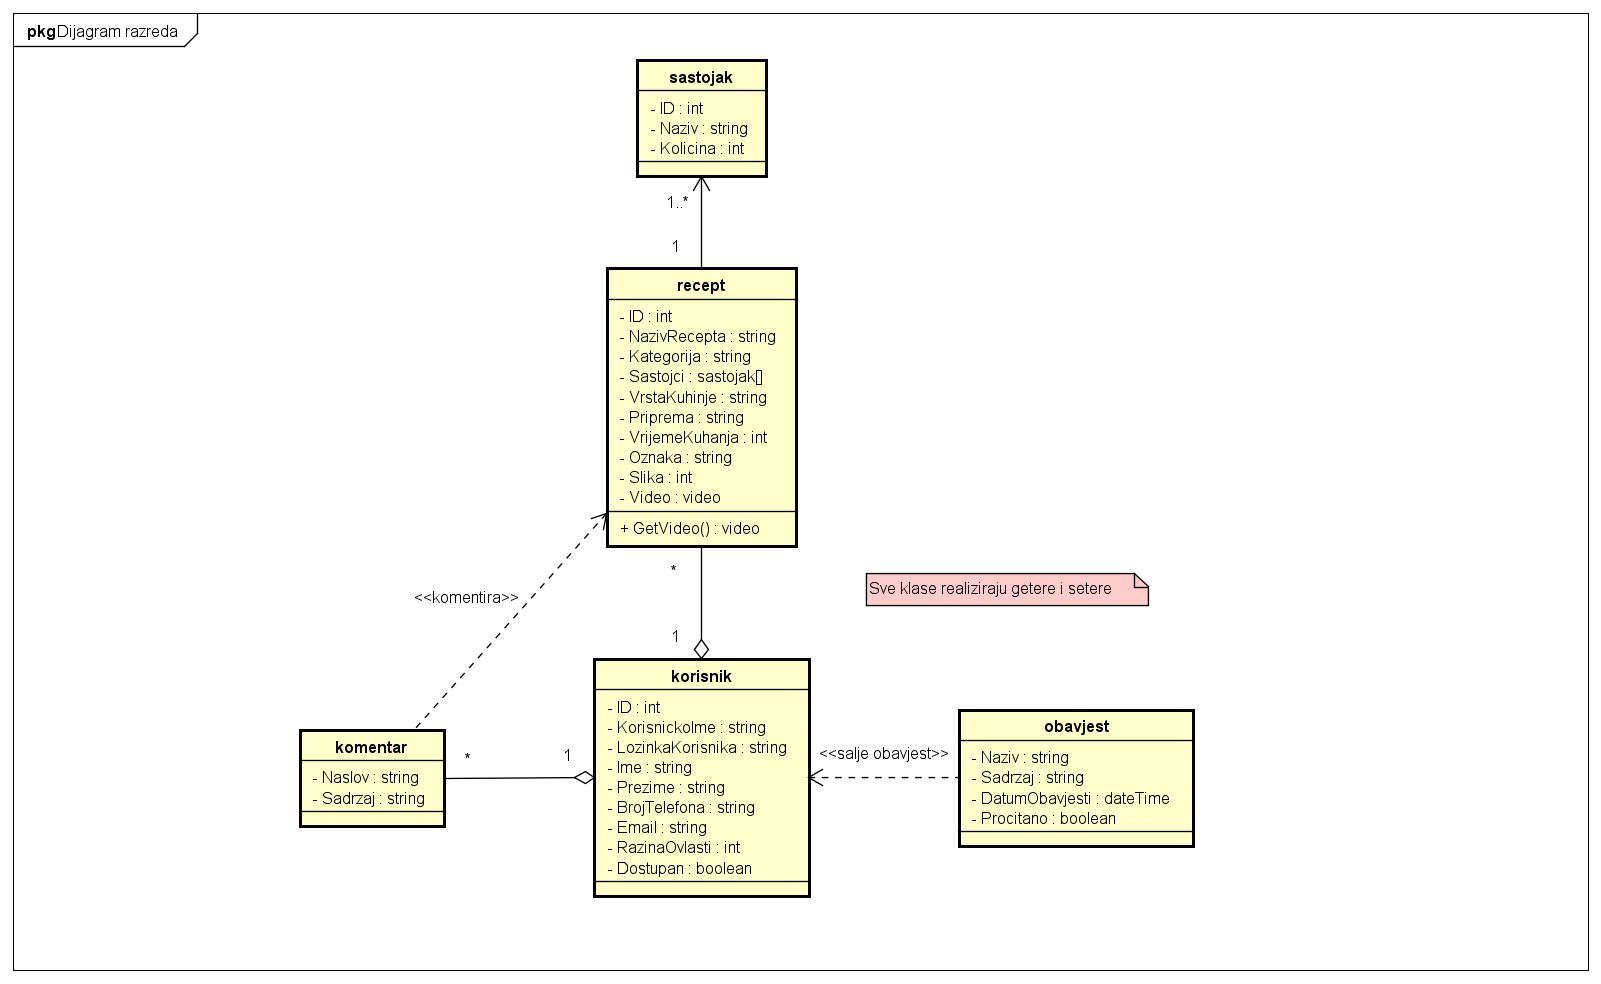
\includegraphics[width=\textwidth]{slike/DijagramRazreda.png} %veličina slike u odnosu na originalnu datoteku i pozicija slike
	\centering
	\caption{Dijagram razreda}
	\label{fig:dijagramraz}
\end{figure}

\begin{figure}[H]
	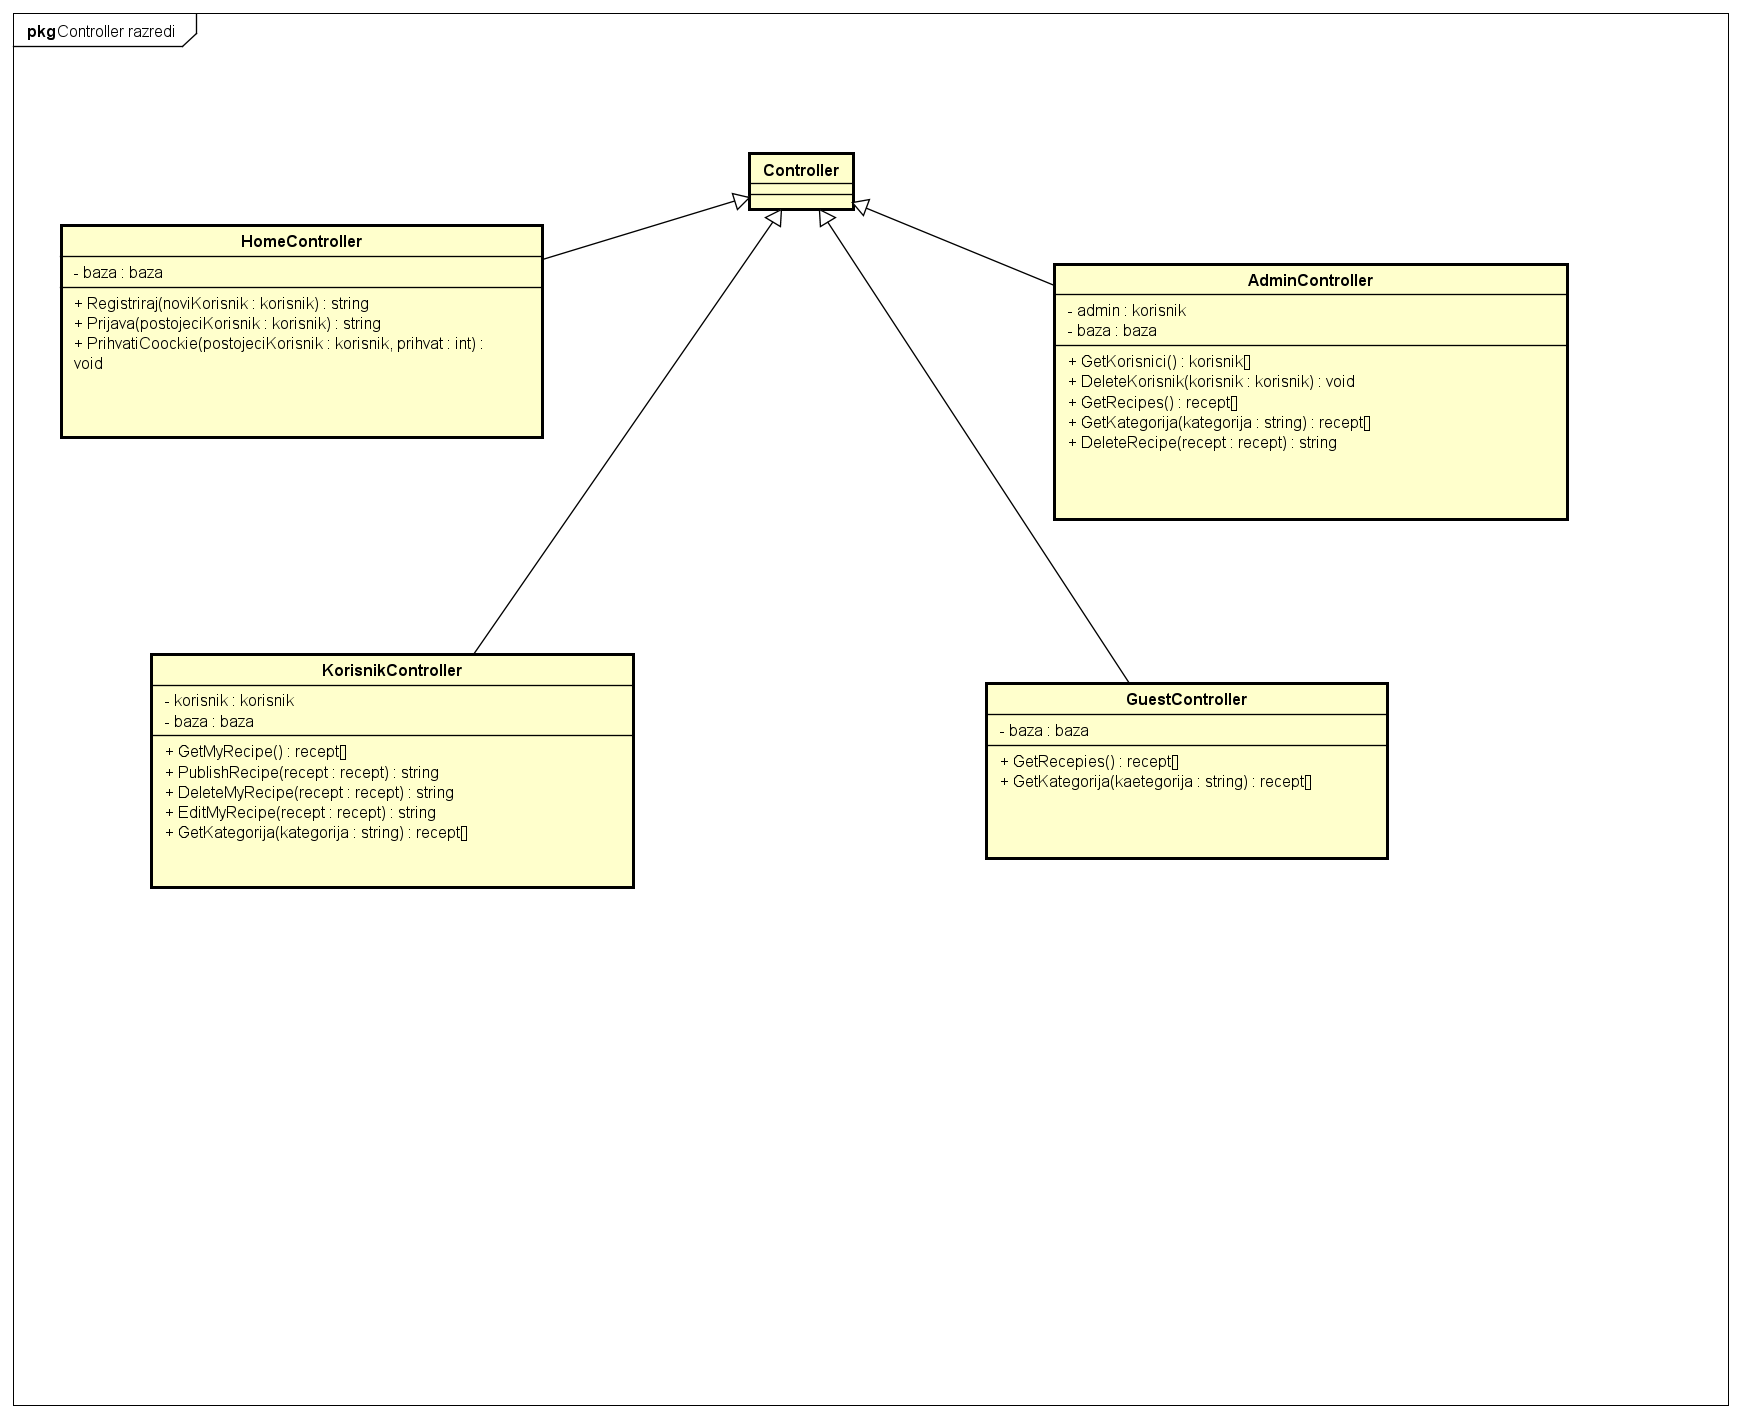
\includegraphics[width=\textwidth]{slike/ControllerRazredi.png} %veličina slike u odnosu na originalnu datoteku i pozicija slike
	\centering
	\caption{Dijagram razreda kontrolera}
	\label{fig:dijagramkontr}
\end{figure}

\begin{figure}[H]
	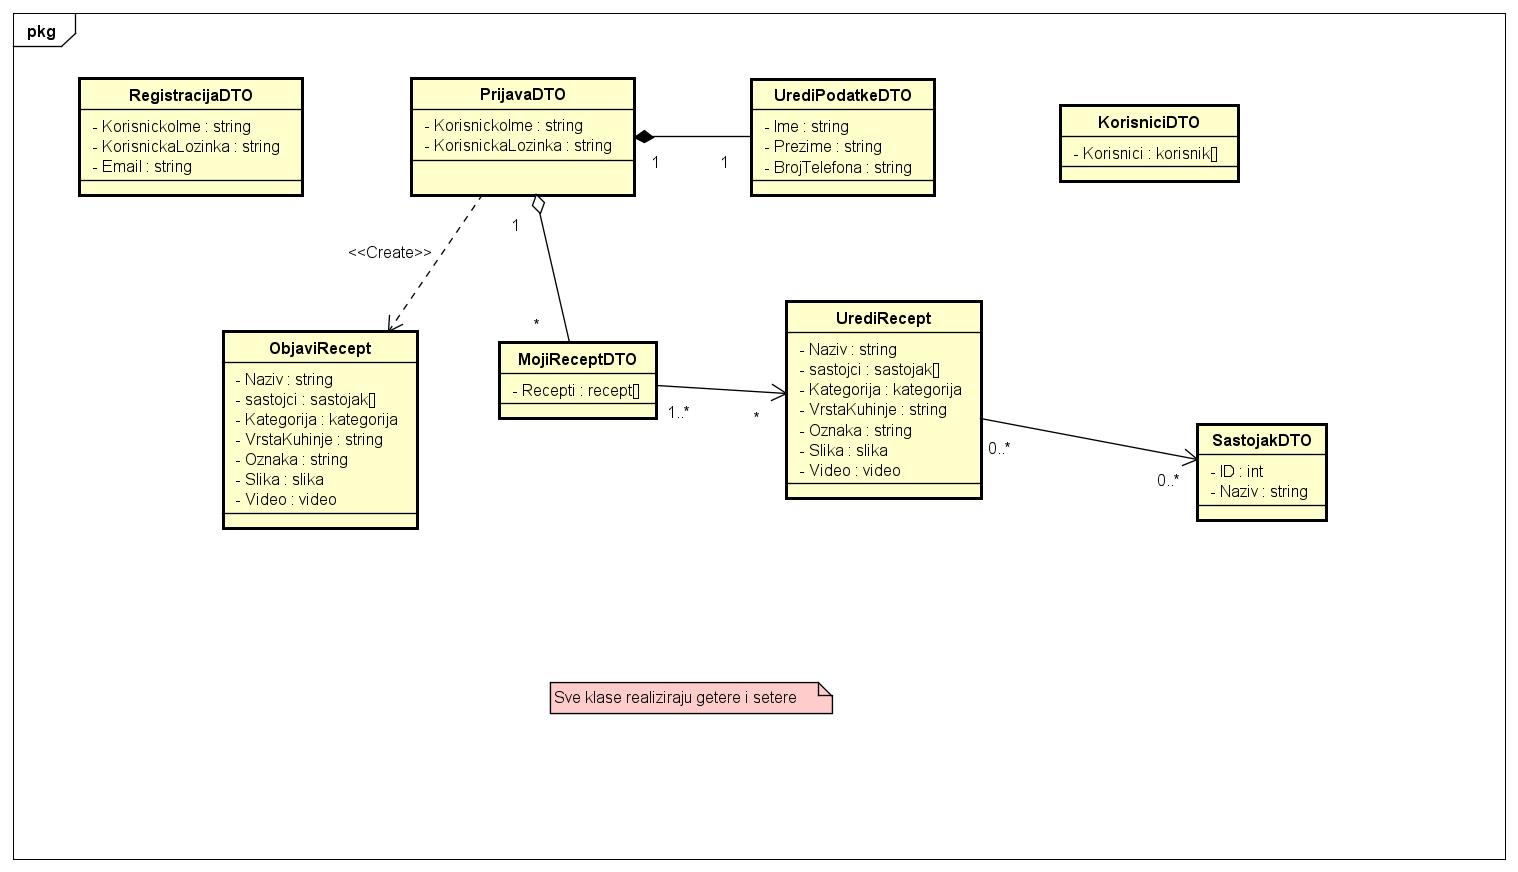
\includegraphics[width=\textwidth]{slike/DTO.png} %veličina slike u odnosu na originalnu datoteku i pozicija slike
	\centering
	\caption{DTO}
	\label{fig:dijagramdto}
\end{figure}

\textbf{\textit{dio 2. revizije}}\\

\textit{Prilikom druge predaje projekta dijagram razreda i opisi moraju odgovarati stvarnom stanju implementacije}



\eject

\section{Dijagram stanja}


\textbf{\textit{dio 2. revizije}}\\

\textit{Potrebno je priložiti dijagram stanja i opisati ga. Dovoljan je jedan dijagram stanja koji prikazuje \textbf{značajan dio funkcionalnosti} sustava. Na primjer, stanja korisničkog sučelja i tijek korištenja neke ključne funkcionalnosti jesu značajan dio sustava, a registracija i prijava nisu. }


\eject

\section{Dijagram aktivnosti}

\textbf{\textit{dio 2. revizije}}\\

\textit{Potrebno je priložiti dijagram aktivnosti s pripadajućim opisom. Dijagram aktivnosti treba prikazivati značajan dio sustava.}

\eject
\section{Dijagram komponenti}

\textbf{\textit{dio 2. revizije}}\\

\textit{Potrebno je priložiti dijagram komponenti s pripadajućim opisom. Dijagram komponenti treba prikazivati strukturu cijele aplikacije.}